\documentclass[nofonts,]{tufte-handout}

% ams
\usepackage{amssymb,amsmath}

\usepackage{ifxetex,ifluatex}
\usepackage{fixltx2e} % provides \textsubscript
\ifnum 0\ifxetex 1\fi\ifluatex 1\fi=0 % if pdftex
  \usepackage[T1]{fontenc}
  \usepackage[utf8]{inputenc}
\else % if luatex or xelatex
  \makeatletter
  \@ifpackageloaded{fontspec}{}{\usepackage{fontspec}}
  \makeatother
  \defaultfontfeatures{Ligatures=TeX,Scale=MatchLowercase}
  \makeatletter
  \@ifpackageloaded{soul}{
     \renewcommand\allcapsspacing[1]{{\addfontfeature{LetterSpace=15}#1}}
     \renewcommand\smallcapsspacing[1]{{\addfontfeature{LetterSpace=10}#1}}
   }{}
  \makeatother
\fi

% graphix
\usepackage{graphicx}
\setkeys{Gin}{width=\linewidth,totalheight=\textheight,keepaspectratio}

% booktabs
\usepackage{booktabs}

% url
\usepackage{url}

% hyperref
\usepackage{hyperref}

% units.
\usepackage{units}


\setcounter{secnumdepth}{2}

% citations
\usepackage{natbib}
\bibliographystyle{plainnat}

%% tint override
\setcitestyle{round} 

% pandoc syntax highlighting

% longtable
\usepackage{longtable,booktabs}

% multiplecol
\usepackage{multicol}

% strikeout
\usepackage[normalem]{ulem}

% morefloats
\usepackage{morefloats}


% tightlist macro required by pandoc >= 1.14
\providecommand{\tightlist}{%
  \setlength{\itemsep}{0pt}\setlength{\parskip}{0pt}}

% title / author / date
\title{TikZ graphics}
\author{Deependra Dhakal}
\date{2020-07-06}

%% -- tint overrides
%% fonts, using roboto (condensed) as default
\usepackage[sfdefault,condensed]{roboto}
%% also nice: \usepackage[default]{lato}

%% colored links, setting 'borrowed' from RJournal.sty with 'Thanks, Achim!'
\RequirePackage{color}
\definecolor{link}{rgb}{0.1,0.1,0.8} %% blue with some grey
\hypersetup{
  colorlinks,%
  citecolor=link,%
  filecolor=link,%
  linkcolor=link,%
  urlcolor=link
}

%% macros
\makeatletter

%% -- tint does not use italics or allcaps in title
\renewcommand{\maketitle}{%     
  \newpage
  \global\@topnum\z@% prevent floats from being placed at the top of the page
  \begingroup
    \setlength{\parindent}{0pt}%
    \setlength{\parskip}{4pt}%
    \let\@@title\@empty
    \let\@@author\@empty
    \let\@@date\@empty
    \ifthenelse{\boolean{@tufte@sfsidenotes}}{%
      %\gdef\@@title{\sffamily\LARGE\allcaps{\@title}\par}%
      %\gdef\@@author{\sffamily\Large\allcaps{\@author}\par}%
      %\gdef\@@date{\sffamily\Large\allcaps{\@date}\par}%
      \gdef\@@title{\begingroup\fontseries{b}\selectfont\LARGE{\@title}\par}%
      \gdef\@@author{\begingroup\fontseries{l}\selectfont\Large{\@author}\par}%
      \gdef\@@date{\begingroup\fontseries{l}\selectfont\Large{\@date}\par}%
    }{%
      %\gdef\@@title{\LARGE\itshape\@title\par}%
      %\gdef\@@author{\Large\itshape\@author\par}%
      %\gdef\@@date{\Large\itshape\@date\par}%
      \gdef\@@title{\begingroup\fontseries{b}\selectfont\LARGE\@title\par\endgroup}%
      \gdef\@@author{\begingroup\fontseries{l}\selectfont\Large\@author\par\endgroup}%
      \gdef\@@date{\begingroup\fontseries{l}\selectfont\Large\@date\par\endgroup}%
    }%
    \@@title
    \@@author
    \@@date
  \endgroup
  \thispagestyle{plain}% suppress the running head
  \tuftebreak% add some space before the text begins
  \@afterindentfalse\@afterheading% suppress indentation of the next paragraph
}

%% -- tint does not use italics or allcaps in section/subsection/paragraph
\titleformat{\section}%
  [hang]% shape
  %{\normalfont\Large\itshape}% format applied to label+text
  {\fontseries{b}\selectfont\Large}% format applied to label+text
  {\thesection}% label
  {1em}% horizontal separation between label and title body
  {}% before the title body
  []% after the title body

\titleformat{\subsection}%
  [hang]% shape
  %{\normalfont\large\itshape}% format applied to label+text
  {\fontseries{m}\selectfont\large}% format applied to label+text
  {\thesubsection}% label
  {1em}% horizontal separation between label and title body
  {}% before the title body
  []% after the title body

\titleformat{\paragraph}%
  [runin]% shape
  %{\normalfont\itshape}% format applied to label+text
  {\fontseries{l}\selectfont}% format applied to label+text
  {\theparagraph}% label
  {1em}% horizontal separation between label and title body
  {}% before the title body
  []% after the title body

%% -- tint does not use italics here either
% Formatting for main TOC (printed in front matter)
% {section} [left] {above} {before w/label} {before w/o label} {filler + page} [after]
\ifthenelse{\boolean{@tufte@toc}}{%
  \titlecontents{part}% FIXME
    [0em] % distance from left margin
    %{\vspace{1.5\baselineskip}\begin{fullwidth}\LARGE\rmfamily\itshape} % above (global formatting of entry)
    {\vspace{1.5\baselineskip}\begin{fullwidth}\fontseries{m}\selectfont\LARGE} % above (global formatting of entry)
    {\contentslabel{2em}} % before w/label (label = ``II'')
    {} % before w/o label
    {\rmfamily\upshape\qquad\thecontentspage} % filler + page (leaders and page num)
    [\end{fullwidth}] % after
  \titlecontents{chapter}%
    [0em] % distance from left margin
    %{\vspace{1.5\baselineskip}\begin{fullwidth}\LARGE\rmfamily\itshape} % above (global formatting of entry)
    {\vspace{1.5\baselineskip}\begin{fullwidth}\fontseries{m}\selectfont\LARGE} % above (global formatting of entry)
    {\hspace*{0em}\contentslabel{2em}} % before w/label (label = ``2'')
    {\hspace*{0em}} % before w/o label
    %{\rmfamily\upshape\qquad\thecontentspage} % filler + page (leaders and page num)
    {\upshape\qquad\thecontentspage} % filler + page (leaders and page num)
    [\end{fullwidth}] % after
  \titlecontents{section}% FIXME
    [0em] % distance from left margin
    %{\vspace{0\baselineskip}\begin{fullwidth}\Large\rmfamily\itshape} % above (global formatting of entry)
    {\vspace{0\baselineskip}\begin{fullwidth}\fontseries{m}\selectfont\Large} % above (global formatting of entry)
    {\hspace*{2em}\contentslabel{2em}} % before w/label (label = ``2.6'')
    {\hspace*{2em}} % before w/o label
    %{\rmfamily\upshape\qquad\thecontentspage} % filler + page (leaders and page num)
    {\upshape\qquad\thecontentspage} % filler + page (leaders and page num)
    [\end{fullwidth}] % after
  \titlecontents{subsection}% FIXME
    [0em] % distance from left margin
    %{\vspace{0\baselineskip}\begin{fullwidth}\large\rmfamily\itshape} % above (global formatting of entry)
    {\vspace{0\baselineskip}\begin{fullwidth}\fontseries{m}\selectfont\large} % above (global formatting of entry)
    {\hspace*{4em}\contentslabel{4em}} % before w/label (label = ``2.6.1'')
    {\hspace*{4em}} % before w/o label
    %{\rmfamily\upshape\qquad\thecontentspage} % filler + page (leaders and page num)
    {\upshape\qquad\thecontentspage} % filler + page (leaders and page num)
    [\end{fullwidth}] % after
  \titlecontents{paragraph}% FIXME
    [0em] % distance from left margin
    %{\vspace{0\baselineskip}\begin{fullwidth}\normalsize\rmfamily\itshape} % above (global formatting of entry)
    {\vspace{0\baselineskip}\begin{fullwidth}\fontseries{m}\selectfont\normalsize\rmfamily} % above (global formatting of entry)
    {\hspace*{6em}\contentslabel{2em}} % before w/label (label = ``2.6.0.0.1'')
    {\hspace*{6em}} % before w/o label
    %{\rmfamily\upshape\qquad\thecontentspage} % filler + page (leaders and page num)
    {\upshape\qquad\thecontentspage} % filler + page (leaders and page num)
    [\end{fullwidth}] % after
}{}

  
\makeatother


\usepackage{booktabs}
\usepackage{longtable}
\usepackage{array}
\usepackage{multirow}
\usepackage{wrapfig}
\usepackage{float}
\usepackage{colortbl}
\usepackage{pdflscape}
\usepackage{tabu}
\usepackage{threeparttable}
\usepackage{threeparttablex}
\usepackage[normalem]{ulem}
\usepackage{makecell}
\usepackage{xcolor}
\usepackage{tikz}
\usepackage{pgfplots}
\pgfplotsset{compat=1.16}
\usepackage{smartdiagram}
\usetikzlibrary{shapes.geometric,intersections,arrows.meta,chains,trees}
\usepackage{sidecap}

\begin{document}

\maketitle




\clearpage

\hypertarget{begining}{%
\section{Begining}\label{begining}}

This document has a two fold purpose -- one, familiarize yourself with
tikz while learning it from basics and second, ease your life with
handful of tricks and packages that do drawing jobs for you. Most of the
ideas are not original and picked up from \url{tex.stackexchange.com}. I
will link to the online contents as we go along with demonstration.
Before anything new, try this very hot manual for pgf at
\url{https://www.iro.umontreal.ca/~simardr/pgfmanual.pdf}. Its 560 pages
full of fun and awesomeness. I think there is barely anything it misses.

One of my first tikz picture included creating just a triangle by
specifying coordinates. Like the one in Figure \ref{fig:raw-triangle}.

\vspace{1cm}

\begin{figure}
\centering
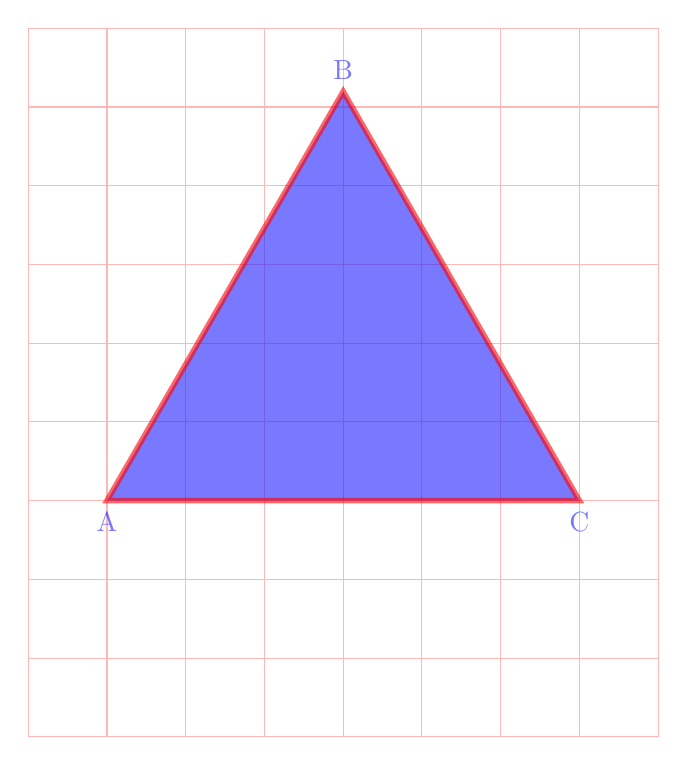
\begin{tikzpicture}
\coordinate (A) at (1,0);
\coordinate (B) at (4,{sqrt(27)});
\coordinate (C) at (7,0);
<!-- % \draw[ddrook gridlines] (0,-3) grid (8,6); -->
<!-- % \draw[ddrook lines, fill, color=blue!88, draw=red, line width=2pt,opacity=0.6] -->
\draw[thin, color=red!28] (0,-3) grid (8,6);
\draw[fill, color=blue!88, draw=red, line width=2pt, opacity=0.6]
(A) node[anchor=north]{A} -- (C) node[anchor=north]{C} -- (B) node[anchor=south]{B} -- cycle;
\end{tikzpicture}
\caption{An equilateral triangle} \label{fig:raw-triangle}
\end{figure}

\hypertarget{more-basic-shapes}{%
\subsection{More basic shapes}\label{more-basic-shapes}}

A basic rectangle geometry is already defined in TikZ. Just input the
starting and ending coordinates.


\begin{tikzpicture}
\fill[red] (0,0) rectangle (1,1);
\end{tikzpicture}

\marginnote{
\begin{tikzpicture}\node[fill=red] at (0,0) {More on this basic shapes and segments in Section \ref{sec:shapes-segments}.};\end{tikzpicture}\newline Note: Tufte/tint by default does not support section numbering and thus not let reference section. We need to fix it by setting 'number\_sections: true' in yaml.}

Next up, we could make potting so much easier is several ways. The same
triangle has been bettered in Figure \ref{fig:triangle-of-breeding}.
Notably, we remove the grid, add dotted segments and improve labelling
of nodes by aligning them.

\vspace{1cm}

\begin{figure}
\centering
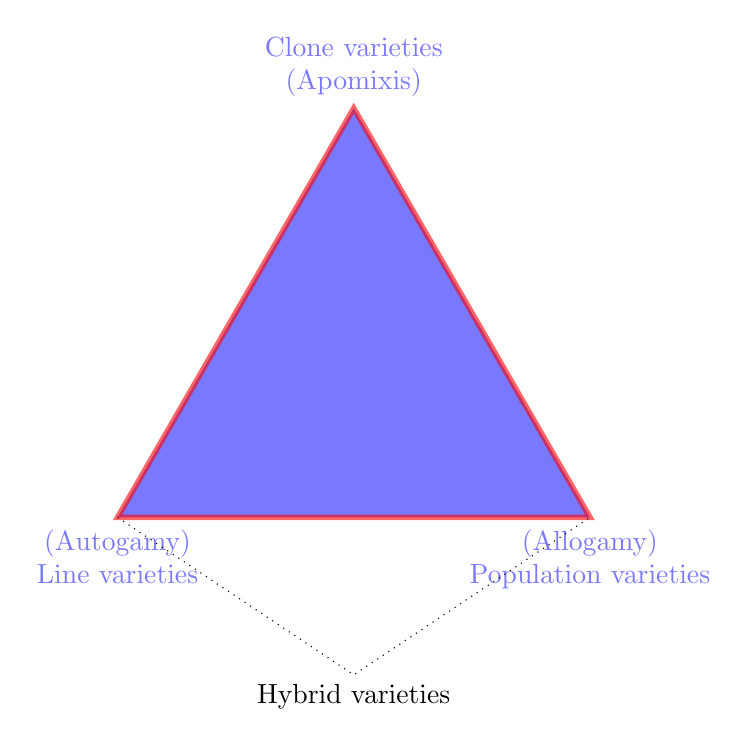
\begin{tikzpicture}
\coordinate (A) at (1,0);
\coordinate (B) at (4,{sqrt(27)});
\coordinate (C) at (7,0);
\draw[fill, color=blue!88, draw=red, line width=2pt,opacity=0.6]
(A) node[anchor=north,align=center]{(Autogamy)\\ Line varieties} -- (C) node[anchor=north,align=center]{(Allogamy)\\ Population varieties} -- (B) node[anchor=south,align=center]{Clone varieties\\ (Apomixis)} -- cycle;
\draw[dotted] (A)--(4,-2) node[anchor=north,align=center]{Hybrid varieties}--(C);
\end{tikzpicture}
\caption{The reproduction triangle with the modes of reproduction (in bracketted letters) and the four breeding categories and resulting types of varieties. The system also imples that thare are not strict barriers between reproductive systems, but a gradual transition from one mode to the neighboring one. Clonal varieties can be selected for strictly apomictic plants. While autogamy and allogamy are not as strict in plant kingdom as even highly autogamous lines may cross fertilize nearby plants. Hybrid breeding, as shown involves both autogamy and allogamy and could be called a man-made breeding system.} \label{fig:triangle-of-breeding}
\end{figure}

\hypertarget{using-intersection-features}{%
\subsection{Using intersection
features}\label{using-intersection-features}}

Using name path requires intersections tikzlibrary

\hypertarget{smartdiagram-template}{%
\subsection{Smartdiagram template}\label{smartdiagram-template}}

But more suited to instant presentation without much hassles. A full pdf
documentation for the Claudio Fiandrino's package is available at
\url{http://texdoc.net/texmf-dist/doc/latex/smartdiagram/smartdiagram.pdf}.
It seems super useful to draw flow diagrams, instantly, alike mermaidjs
graphics. More popular drawing types are: descriptive diagram, priority
descriptive diagram, constellation diagram, sequence diagram, flow
diagram, circular diagram, etc.

\smartdiagram[priority descriptive diagram]{
  Develop a document structure,
  Choose a document class,
  Select suitable packages,
  Setup the document preamble,
  Write your document,
  Finetune the layout}

\begin{center}
\smartdiagramset{border color=none,
  uniform color list=teal!60 for 4 items,
  arrow style=[-stealth,
  module x sep=3.75,
  back arrow distance=0.75,
  }
\smartdiagram[flow diagram:horizontal]{Set up,Run,Analyse,Modify~/ Add}
\end{center}

\clearpage

\hypertarget{using-chains-and-flows}{%
\subsection{Using chains and flows}\label{using-chains-and-flows}}

\begin{figure}
\centering
\resizebox{0.9\textwidth}{!}{%
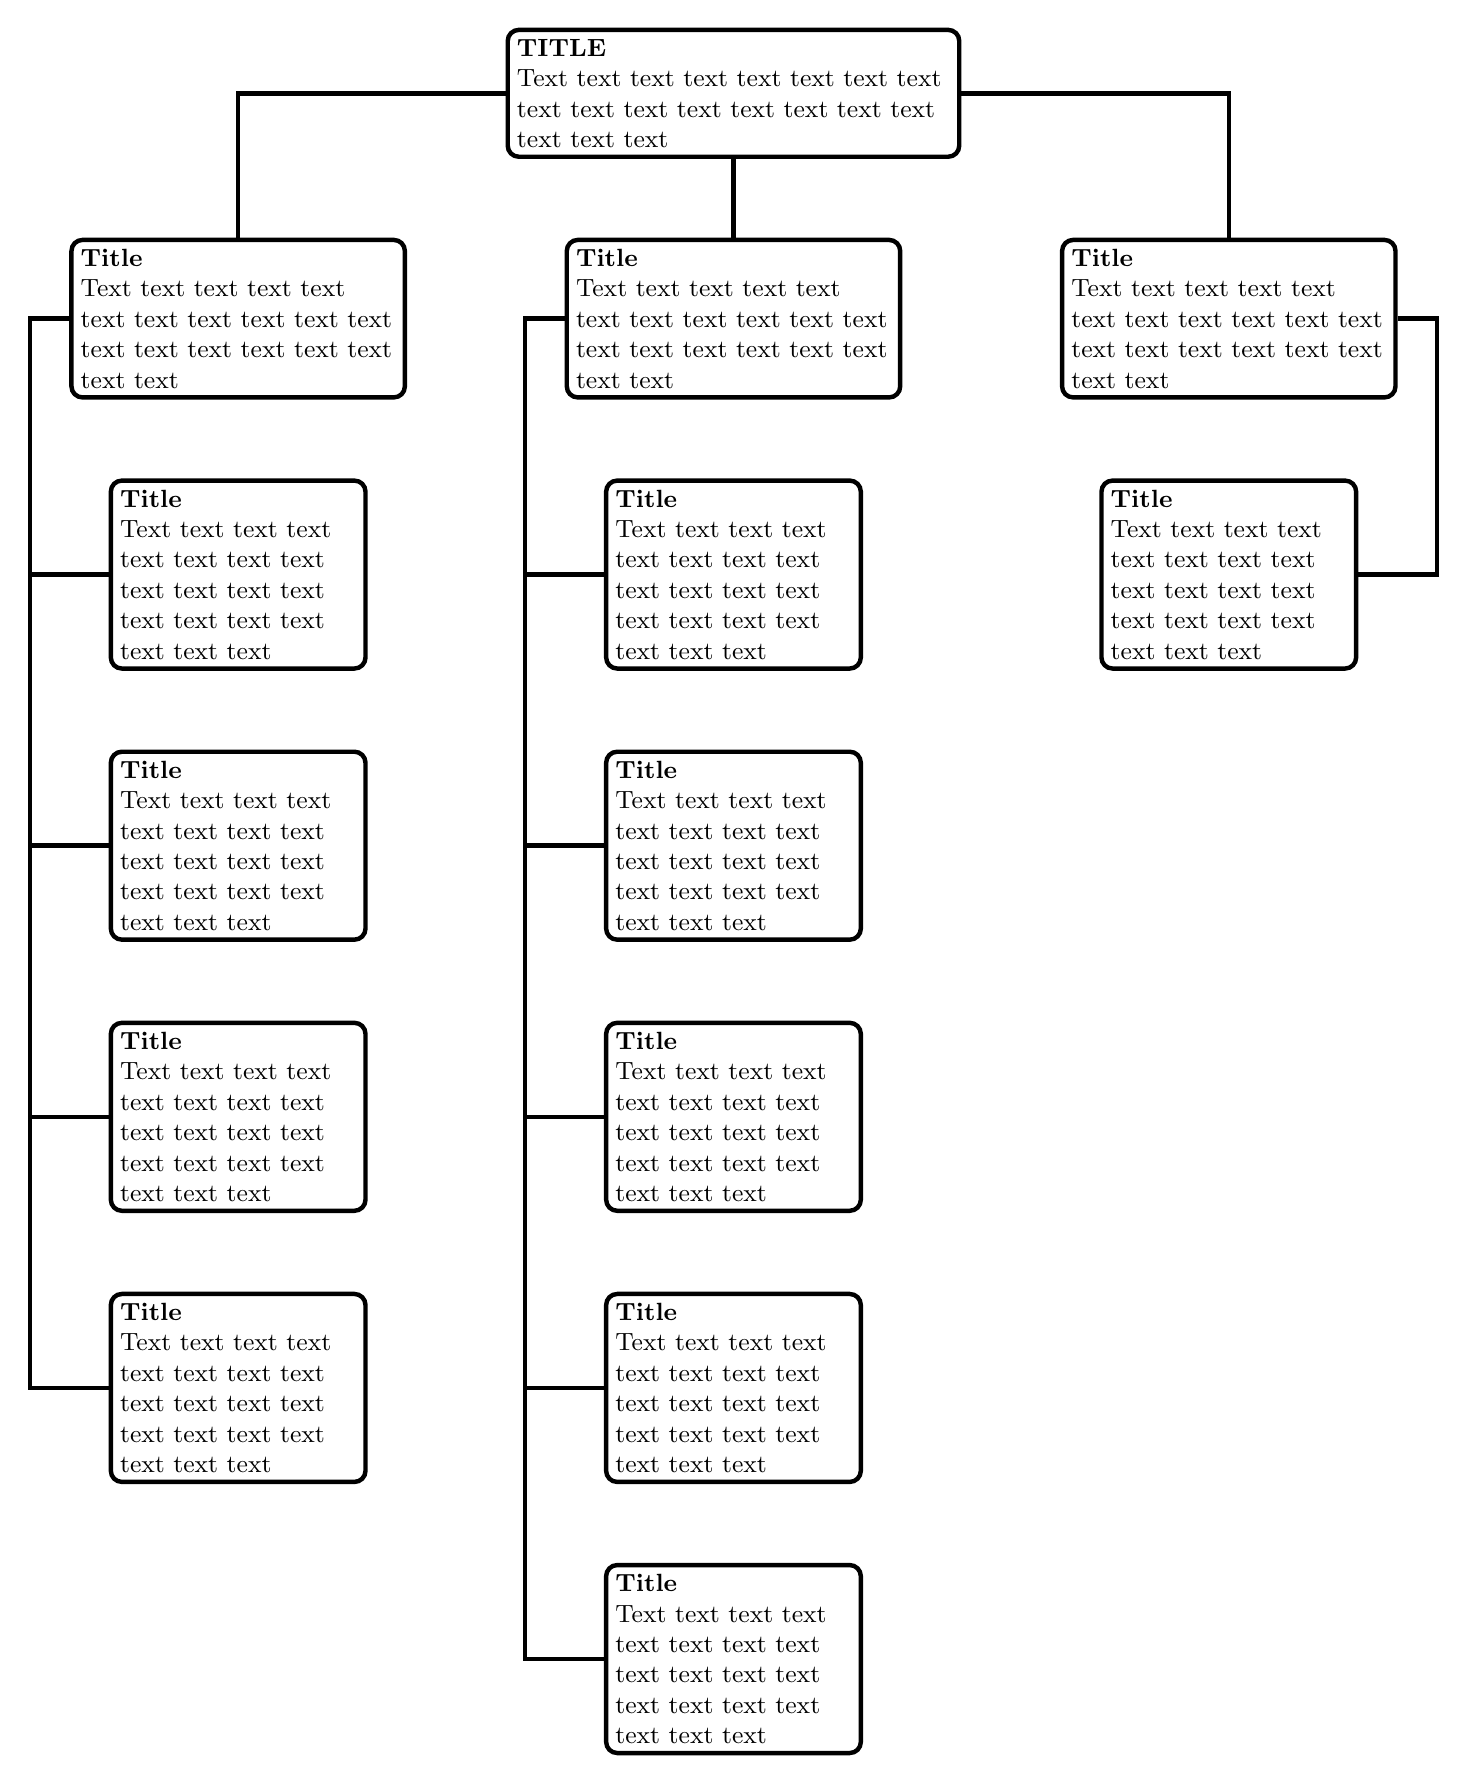
\begin{tikzpicture}[
  ultra thick,
  node distance=1cm and 2cm,
  every node/.append style={
    draw,
    rounded corners,
    align=left,
    font=\small
  },
  top node/.style={text width=+55mm},
  wide node/.style={text width=+40mm},
  thin node/.style={text width=+30mm},
  start chain/.list={ch1 going below, ch2 going below, ch3 going below}
]

\node[top node](problema) {\textbf{TITLE}\\ Text text text text text text text text text text text text text text text text text text text};

\begin{scope}[every node/.append style={wide node}]
  \node[below=of problema, on chain=ch2] (causa2) {\textbf{Title}\\ Text text text text text text text text text text text text text text text text text text text};
  \node[left=of causa2   , on chain=ch1] (causa1) {\textbf{Title}\\ Text text text text text text text text text text text text text text text text text text text};
  \node[right=of causa2  , on chain=ch3] (causa3) {\textbf{Title}\\ Text text text text text text text text text text text text text text text text text text text};
\end{scope}
\begin{scope}[
  every node/.append style={thin node},
  place nodes on chain and install special path/.style n args={3}{
  every node/.append style={on chain=#1,join},
  every join/.append style={to path=(#1-begin.#3) #2 (\tikztotarget)}
}
]
  \begin{scope}[place nodes on chain and install special path={ch1}{-- ++(left:.5cm) |-}{west}]
    \node {\textbf{Title}\\ Text text text text text text text text text text text text text text text text text text text};
    \node {\textbf{Title}\\ Text text text text text text text text text text text text text text text text text text text};
    \node {\textbf{Title}\\ Text text text text text text text text text text text text text text text text text text text};
    \node {\textbf{Title}\\ Text text text text text text text text text text text text text text text text text text text};
  \end{scope}
  \begin{scope}[place nodes on chain and install special path={ch2}{-- ++(left:.5cm) |-}{west}]
    \node {\textbf{Title}\\ Text text text text text text text text text text text text text text text text text text text};
    \node {\textbf{Title}\\ Text text text text text text text text text text text text text text text text text text text};
    \node {\textbf{Title}\\ Text text text text text text text text text text text text text text text text text text text};
    \node {\textbf{Title}\\ Text text text text text text text text text text text text text text text text text text text};
    \node {\textbf{Title}\\ Text text text text text text text text text text text text text text text text text text text};
  \end{scope}
  \begin{scope}[place nodes on chain and install special path={ch3}{-- ++(right:.5cm) |-}{east}]
    \node {\textbf{Title}\\ Text text text text text text text text text text text text text text text text text text text};
  \end{scope}
\end{scope}

\draw (problema) -| (causa1);
\draw (problema) -- (causa2);
\draw (problema) -| (causa3);
\end{tikzpicture}
}%
\caption{This figure uses chains tikzlibrary and in addition, can be simplified a bit using paths.ortho tikzlibrary. The latter library is not available by default and is detailed at \url{https://tex.stackexchange.com/a/121121/133229}}. Notice how enclosing the picture in resizebox places it correctly within the bounds of textwidth.
\label{fig:flow-chains}.
\end{figure}

Use of flow and chain diagrams is easily apparent\footnote{Figure
  \ref{fig:flow-chains} can be heavily customized}.

\hypertarget{tikz-tree-diagram}{%
\subsection{TikZ tree diagram}\label{tikz-tree-diagram}}

This diagram is drawn from
\url{https://tex.stackexchange.com/a/161263/133229}. As an alternative
to tikz library \texttt{trees}, \texttt{forest} package is also
suggested. But we stick to the basics and add the \texttt{trees}
tikzlibrary to the header.

\resizebox{\textwidth}{!}{%
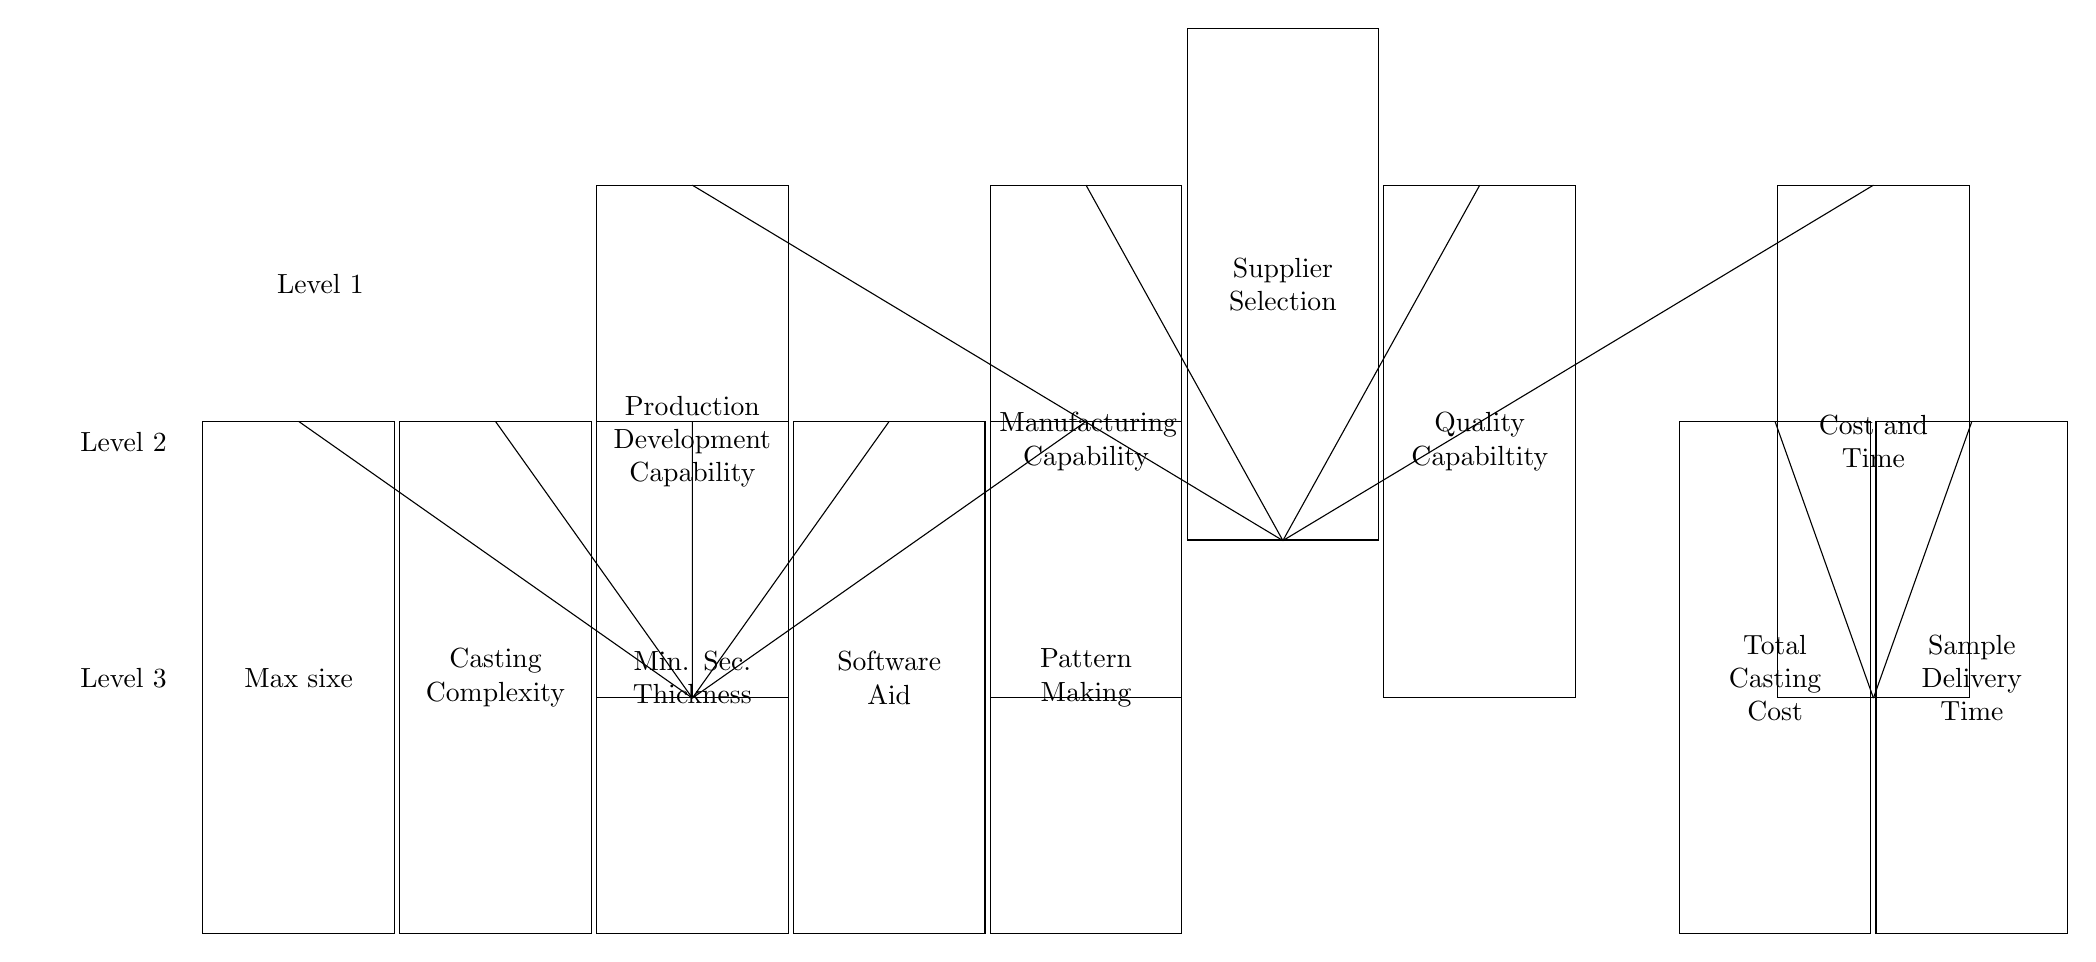
\begin{tikzpicture}
  %[auto,every node/.style={rectangle,draw, text centered, text width=2.2cm,minimum height=1.5cm },node distance=6cm]
  [auto,every node/.style={rectangle,draw, text centered, text width=2.2cm,minimum height=6.5cm },node distance=12cm]
\tikzset{%
level 1/.style={sibling distance = 5cm, level distance=2cm,edge from parent path={(\tikzparentnode.south) -- (\tikzchildnode.north)}},
level 2/.style={sibling distance = 2.5cm,level distance=3cm}
}
  \node (0){Supplier \\ Selection}
    child {node (1) {Production \\ Development \\Capability}
              child {node (2) {Max sixe}}
              child {node {Casting\\Complexity}}
              child {node {Min. Sec.\\Thickness}}
              child {node {Software\\Aid}}
              child {node {Pattern\\Making}}}
    child {node {Manufacturing\\Capability}}
    child {node {Quality\\Capabiltity}}
    child {node {Cost and\\Time}
              child {node {Total\\ Casting\\ Cost}}
              child {node {Sample\\Delivery\\Time}}};
\node at (0) [xshift=-11cm,left,draw=none]{Level 1};
\node at (1) [xshift=-6cm, left,draw=none]{Level 2};
\node at (2) [xshift=-1cm, left,draw=none]{Level 3};
\end{tikzpicture}
}

\hypertarget{drawing-probability-trees}{%
\subsection{Drawing probability trees}\label{drawing-probability-trees}}

Probability trees can be drawn using both the forest package and usign
\texttt{\textbackslash{}usetikzlibrary\{trees\}}.

\tikzset{%
  level 1/.style={level distance=3.5cm, sibling distance=4.5cm},
  level 2/.style={level distance=3.5cm, sibling distance=2cm},
  bag/.style={text width=50pt, text centered},
  end/.style={circle, minimum width=3pt, fill, inner sep=0pt},
}
\begin{tikzpicture}[grow=right, sloped]
  \node[bag] {Urn $3G, 4R, 2W$}
  child {
    node[bag] {$2G, 4R, 2W$}
    child {
      node[end, label=right: {$P(G_1\cap G_2)=\frac{1}{3}\times\frac{1}{4}=\frac{1}{12}$}] {}
      edge from parent
      node[above] {$G$}
      node[below]  {$\frac{1}{4}$}
    }
    child {
      node[end, label=right: {$P(G_1\cap R_2)=\frac{1}{3}\times\frac{1}{2}=\frac{1}{6}$}] {}
      edge from parent
      node[above] {$R$}
      node[below]  {$\frac{1}{2}$}
    }
    child {
      node[end, label=right: {$P(G_1\cap W_2)=\frac{1}{3}\times\frac{1}{4}=\frac{1}{12}$}] {}
      edge from parent
      node[above] {$W$}
      node[below]  {$\frac{1}{4}$}
    }
    edge from parent
    node[above] {$G$}
    node[below]  {$\frac{1}{3}$}
  }
  child {
    node[bag] {$3G, 3R, 2W$}
    child {
      node[end, label=right: {$P(R_1\cap G_2)=\frac{4}{9}\times\frac{3}{8}=\frac{2}{5}$}] {}
      edge from parent
      node[above] {$G$}
      node[below]  {$\frac{3}{8}$}
    }
    child {
      node[end, label=right: {$P(R_1\cap R_2)=\frac{4}{9}\times\frac{3}{8}=\frac{4}{15}$}] {}
      edge from parent
      node[above] {$R$}
      node[below]  {$\frac{3}{8}$}
    }
    child {
      node[end, label=right: {$P(R_1\cap W_2)=\frac{4}{9}\times\frac{1}{4}=\frac{4}{15}$}] {}
      edge from parent
      node[above] {$W$}
      node[below]  {$\frac{1}{4}$}
    }
    edge from parent
    node[above] {$R$}
    node[below]  {$\frac{4}{9}$}
  }
  child {
    node[bag] {$3G, 4R, 1W$}
    child {
      node[end, label=right: {$P(W_1\cap G_2)=\frac{2}{9}\times\frac{3}{8}=\frac{1}{12}$}] {}
      edge from parent
      node[above] {$G$}
      node[below]  {$\frac{3}{8}$}
    }
    child {
      node[end, label=right: {$P(W_1\cap R_2)=\frac{2}{9}\times\frac{1}{2}=\frac{1}{9}$}] {}
      edge from parent
      node[above] {$R$}
      node[below]  {$\frac{1}{2}$}
    }
    child {
      node[end, label=right: {$P(W_1\cap W_2)=\frac{2}{9}\times\frac{1}{8}=\frac{1}{36}$}] {}
      edge from parent
      node[above] {$W$}
      node[below]  {$\frac{1}{8}$}
    }
    edge from parent
    node[above] {$W$}
    node[below]  {$\frac{2}{9}$}
  };
\end{tikzpicture}

\hypertarget{side-caption-plot-uses-sidecap-package}{%
\subsection{Side caption plot (uses sidecap
package)}\label{side-caption-plot-uses-sidecap-package}}

\begin{SCfigure}[\sidecaptionrelwidth][t!]
    \centering
        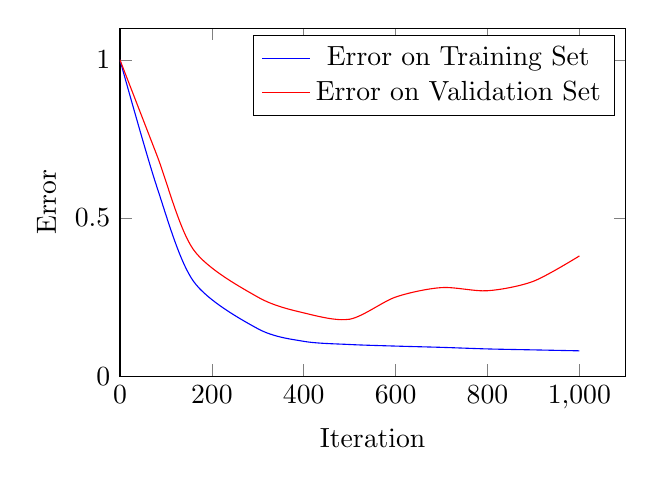
\begin{tikzpicture}
        \begin{axis}[height=6cm,width=8cm,ylabel=Error,xlabel=Iteration,xmin=0,ymin=0]
            \addplot[blue,smooth] coordinates{(0,1)(80,0.6)(160,0.3)(300,0.15)(400,0.11)(500,0.1)(600,0.095)(700,0.091)(800,0.086)(900,0.083)(1000,0.08)};
            \addlegendentry{Error on Training Set}
            \addplot[red,smooth] coordinates{(0,1)(80,0.7)(160,0.4)(300,0.25)(400,0.2)(500,0.18)(600,0.25)(700,0.28)(800,0.27)(900,0.3)(1000,0.38)};
            \addlegendentry{Error on Validation Set}
        \end{axis}
    \end{tikzpicture}
        \caption[Early stopping based on a validation set.]{The error on the validation set (red) is usually getting larger when the network begins to overfit the training set. Thus, although the error on the training set (blue) is decreasing monotonically, we may want to stop training early to avoid overfitting.}
        \label{fig:early-stopping}
\end{SCfigure}

\hypertarget{sec:shapes-segments}{%
\subsection{Shapes and segments}\label{sec:shapes-segments}}



\end{document}
